% -----------
% SETUP
% -----------
\documentclass{physics_article_B}
\title{Mechanical Vibrations of Droplets in Fluidic Systems}
\mytitle{Mechanical Vibrations of Droplets in Fluidic Systems}
\myname{Dominic Coy \& Oliver Gordon}
\studentid{4227789 \& 4224942}
\date{Due Date: 1 June 2018}
\setlength{\bibsep}{10pt plus 0.3ex}
\begin{document}
	
% ----------------------
% COVERSHEET
% ----------------------
\pagenumbering{roman} 
\setcounter{page}{0}
%\includepdf[scale=1]{Images/Cover.pdf}
%\maketitle

% ----------------------
% ABSTRACT
% ----------------------
\pagenumbering{gobble} 
\begin{abstract}
	\large{Insert the geratest abstract ever written 
}
\end{abstract}
	
% ----------------------
% CONTENTS
% ----------------------
%\vspace{4cm}

\tableofcontents

\pagenumbering{roman} 
\setcounter{page}{1}
\setlength{\parskip}{8pt}  
% ----------------------
% INTRODUCTION
% ----------------------
\newpage
\pagenumbering{arabic} 
\setcounter{page}{1}

\section{Introduction\label{sect:intro}}

    Simultaneously measuring the rheological properties of fluids, such as viscosity and surface tension, has, in the past, been accomplished with rheometers\textsuperscript{\cite{harrold2}} or drop volume techniques\textsuperscript{\cite{harrold2}}. However, these methods are not particularly viable when analysing rare or expensive fluids, such as blood droplets in forensics, as they require large volumes of a fluid. When only a few millilitres of a fluid is available, the most promising analysis method is to induce oscillations in small droplets\textsuperscript{\cite{harrold}}, and analyse how these oscillations refract a laser through the droplet using a photodiode. Other applications of this vibrational method and supporting theory include monitoring inkjet printing performance\cite{Martin2008}, simulating the crustal deformation of planets\cite{vukasinovic}, and studying energy relaxation in stars\cite{vukasinovic}.
    
    Early experiments using droplets in rheology were based on theoretical models developed by Rayleigh\textsuperscript{\cite{rayleigh}} and Chandrasekhar\textsuperscript{\cite{chandrasekhar2}} who showed that, by using simple equations, vibrational frequencies of droplets were related to the viscosity and surface tension of a free liquid globe (essentially a levitated droplet). Temperton et al. claimed to be the first to present a combined theoretical and experimental study of simple Newtonian fluids, such as water, in 2014\textsuperscript{\cite{temperton}}. This approach was later extended by multiple authors who demonstrated that, provided surface tension is already known, this technique could be used to extract frequency dependent physical properties of viscoelastic droplets, such as blood\textsuperscript{\cite{egry}}. 
    
    Although multiple previous authors have demonstrated the viability of manual testing, this is not ideal. As such, this project aimed to develop a proof of concept system to automate this process. This involved building a high-throughput system (an automated system so that large scale repetition of an experiment is feasible) to consistently create and transport spherical droplets suspended in oil. The droplets were then oscillated and analysed, with a laser and photodiode, to determine their rheological properties.
    
    In the future the ability to track the properties of a fluid in real time using a high-throughput system which was first investigated by Harrold et al. in 2016\cite{harrold}. A system such as this could be applied to lab-on-a-chip systems, such as inexpensive, reliable tests\textsuperscript{\cite{yager}} for medical diagnosis. Furthermore, droplets containing mixed fluids could also be investigated along with simultaneously measuring the interfacial tension between both the droplets and the carrier fluid\textsuperscript{\cite{Backholm2017}}.
    
    In this paper the history of the field is discussed, along with the associated theory. Next, the techniques used to locate the droplets and determine their size are covered. The 4 different methods used to attempt to induce oscillations are debated, followed by an explanation on how the system was automated. The validity of this system is demonstrated using distilled water, before discussing the results of the project and their implications. Finally, future improvements that could have been made to the project and future directions to take the research are discussed.

% ----------------------
% Literature Review
% ----------------------
\section{Literature Review\label{sect:lit}}

    Building on the work by Rayleigh in 1879, which related the frequency of oscillation of fluidic jets with their area and pressure\textsuperscript{\cite{rayleigh}}, in 1932 Lamb et al. derived an expression for the oscillation frequency of inviscid droplets in an inviscid fluid. Lamb et al. also derived approximate expressions for the rate of damping of oscillations in a viscous droplet in an inviscid fluid and for the oscillations of a bubble of gas in a low viscosity liquid. In their derivations, the velocity fields found for small oscillations of an inviscid fluid were used to estimate the rate of viscous dissipation (the rate that shear forces turn work done by a fluid on adjacent layers into heat) in a droplet with small viscosity\textsuperscript{\cite{lamb}}. Then, in 1960, Reid analysed the oscillations of a viscous droplet in a low-density gas or a vacuum\textsuperscript{\cite{reid}}. His experiment and analysis were summarised in the book Hydrodynamics and Hydrodynamic Stability by Chandrasekhar in 1961\textsuperscript{\cite{chandrasekhar}}. In 1965, Velentine et al. used the same methods as Lamb et al. to derive expressions for the damping rate of oscillations when a low viscosity droplet was submerged in a low viscosity fluid\textsuperscript{\cite{velentine}}. In 1968, Miller et al. derived a general dispersion equation for the oscillations of viscous droplets immersed in a viscous fluid, which could also be applied when the interface between the two fluids possessed elastic and viscous properties of its own. They also derived equations for the rate of damping of oscillations and frequency for specific cases including when the interface between the two fluids is free or is inextensible\textsuperscript{\cite{miller}}.
    
    Since then, experiments have focused on a variety of droplet shapes. Two of the three common droplet geometries are sessile (lying on a surface)\cite{Temperton2012, vukasinovic, Backholm2017} and pendant (teardrop-shaped and suspended off a surface such as a needle)\cite{Temperton2012}. Despite the relative experimental ease of investigating these suspended droplets, damping interactions and droplet shape can be influenced by the suspension surface\cite{Sharp2011}. This alters the vibrational spectra of the droplets, producing errors yet to be fully rectified\cite{harrold}. Despite this, many authors limit such experiments to sessile droplets a single surface\cite{Sharp2011}, leading to differing results. These mechanisms can be partly avoided by using either superhydrophobic or superamphiphobic surfaces as the droplets take on a more spherical shape and can be described with similar equations to levitated droplets derived by Miller et al. There is therefore an impetus to find a reliable method to create fully spherical droplets.
    
    Much of the initial research within the area of spherical droplets was driven by the ambition to study containerless crystallisation of pure liquids in microgravity\textsuperscript{\cite{wilkes}}. However, much of the current research has been focused on the determination of the rheological properties of the droplets. Although it is possible to investigate large spherical droplets by performing the experiment in low gravity (as done in 1979\cite{holt} on Space Shuttle Columbia), this is impractical in this project. Therefore, a wide variety of alternative methods for levitating droplets, other than using microgravity, have been considered. Methods that have been used to levitate the droplets include magnetic\textsuperscript{\cite{temperton, hill}}, electrostatic\textsuperscript{\cite{mugele, wong}}, acoustic\textsuperscript{\cite{trinh, Yarin1998}} and aerodynamic\textsuperscript{\cite{benmore}}. Alternatively, McHale et al. demonstrated the feasibility of determining rheological properties of levitated droplets by using vibrating liquid marbles (droplets stabilised by the adsorption of small particles). However, they found that the small particles dominated the droplet's physical properties and so the application of this approach was limited\textsuperscript{\cite{mchale}}. Therefore, there is a great interest in analysing droplets suspended within another fluid as the droplets do not need to be stabilised by the adsorption of small particles and hence, act like levitated droplets. This is achieved by placing a droplet of fluid within a suspension medium of different viscosity. 
    
    One of the main advantages of suspending a droplet within another fluid over other methods of levitation is a lower mass loss. During an experiment, mass will be lost as the droplet evaporates over time. When suspended within another fluid, this has been shown to be 2-4\%, which is significantly lower than for other methods which see over 10\% \cite{harrold2} mass loss. However, to the best of our knowledge no author has modelled this mass loss and taken it into account. Furthermore, the way in which mass is calculated is also very basic; the droplet is weighed before and after an experiment by comparing the mass of a syringe or paper towel both with and without the droplet. These methods do not take into account leftover residue, and in the case of paper towels are destructive. Additionally, other methods of levitation requires placing droplets by hand, which is a slow process. There is therefore a significant impetus to develop a high throughput system allowing multiple droplets, suspended within another fluid, to be quickly analysed automatically.

\section{Theory\label{sect:theory}}

    Following on from prior work, the major assumption was taken that the droplets analysed in this experiment were perfectly spherical. This is because the lowest energy state (and therefore shape) of a droplet was influenced by its surface tension, $\gamma$, and gravitational interactions, $g_{eff}$. $\gamma$ made the droplet spherical, whilst $g_{eff}$ distorted it. Because these two interactions opposed each other, there existed a critical droplet radius at which its shape changed from spherical to distorted. This was the capillary length, $l_{cap}$, and was defined by the equation\cite{temperton},
        
        \begin{equation} 
        \label{eq:lcap}
            l_{cap} = \sqrt{\frac{\gamma }{\rho g_{eff} }}, 
        \end{equation}
    
    where $\rho$ was the density of the droplet. It was therefore assumed that a droplet was spherical if it has radius, $R$, lower than its capillary length $l_{cap}$. However, as $l_{cap}$ was not always known, it was imperative that droplets were kept as small as possible during the project. 

    As the droplet had an equilibrium state, it would undergo shape oscillations when a small perturbation was applied\cite{oscillate}. If this perturbation was in the form of an impulse, the surface of the droplet would be driven at all frequencies (owing to the mathematics of Fourier transforming a delta function). The vibrations not at the resonant frequency were damped, leaving only the vibrations at the resonant frequency of the droplet with a non-zero amplitude. For optimal results, it had been shown that any applied impulse must be long enough to give sufficient time to perturb the drop, but short enough to still be an impulse and not drive the droplet at a particular frequency\cite{temperton}. Furthermore, the amplitude of oscillations must be kept to under 0.1$R$, following work from Becker et al. who found that above this limit oscillations become non-linear, causing the simple equations used here to fail\cite{becker}.
    
    These oscillations decayed exponentially, giving a time dependant signal such as the one shown in Figure \ref{fig:temperton:signal}. The power spectral density was then obtained by Fourier transforming this signal, and is shown in Figure \ref{fig:temperton:PD}. The remaining resonant frequencies correspond to different modes, $n$, of oscillation. The $n=1$ node corresponds to oscillations of the droplet's centre of mass\textsuperscript{\cite{miller}}, whilst the $n\geq2$ nodes correspond to the surface oscillations which were the focus of interest in this project. The corresponding frequency, $f_n$, and full-width-half-maxima, $\Delta f_n$, was then extracted from the power spectral density. 

        \begin{figure}[H]
            \centering
                \begin{subfigure}[b]{0.48\textwidth}\hspace*{0cm}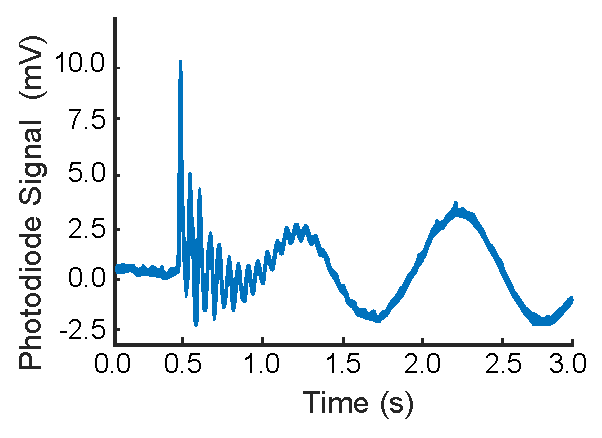
\includegraphics[width=\textwidth]{Figures/TempertonSignal.eps}
                    \caption{Original Signal}
                    \label{fig:temperton:signal}
                \end{subfigure}\hspace{3pt}
                \begin{subfigure}[b]{0.48\textwidth}\hspace*{0cm}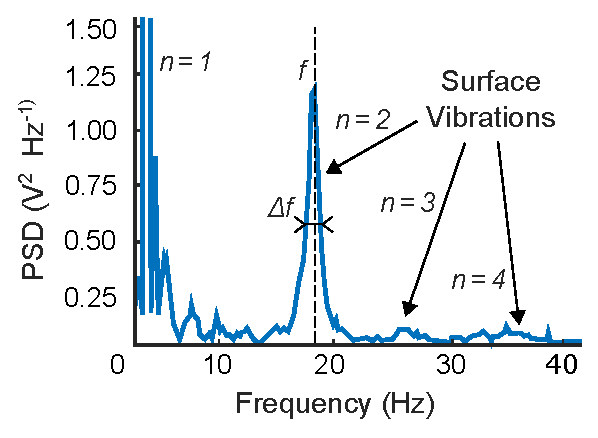
\includegraphics[width=\textwidth]{Figures/TempertonSignalPD.eps}
                    \caption{Fourier Transform}
                    \label{fig:temperton:PD}
                \end{subfigure}
            \caption{Figure to demonstrate (a) the time dependant signal produced when oscillating a droplet of water with an impulse, and (b) its resulting Fourier Transform. The resonant vibrations on the surface of the droplet can be seen in (a) as the initial, rapidly oscillating components of the signal. These correspond to multiple nodes, $n$, of oscillation in (b). The frequency, $f$, and full-width-half-maxima, $\Delta f$, can then be used to determine the rheological properties of the droplet. Adapted from Temperton et. al.\cite{temperton}}\label{fig:temperton}
        \end{figure}

    The surface tension, $\gamma$, and viscosity, $\eta$, of the fluid was then calculated using the equations,
 
        \begin{equation} 
        \label{eq:SurfaceTension}
            \gamma = \frac{4\rho R^{2}}{\pi n^{2}}(\Delta f^{2} + f^{2}),
        \end{equation}
        
        \begin{equation} 
        \label{eq:Viscosity}
            \eta = \frac{\pi \rho \Delta f R^{2}}{n^{2}},
        \end{equation}

    where $\rho$ is the density of the droplet. For pure water in air, it was expected that\cite{expected1} $\gamma$ = 72.80 mNm$^{-1}$ and\cite{expected2} $\eta$ = 8.94 x 10$^{-4}$ Nm$^{2}$s$^{-1}$. However, these values and equations do not perfectly apply to the water in oil used in this experiment. In the absense of a complete theory, they therefore served as a guideline to the values expected to be obtained. 
    
    To determine $R$, checkerboards of known dimensions were used to map the pixels on a screen to real world space. Because cameras have no depth-perception, this required the assumption that the object of interest was in the same plane as the checkerboard. Once the height and width of a spherical droplet, $R_x$ and $R_y$ respectively, was found in an image containing a checkerboard, $R$ was calculated with simple trigonometry,
            
        \begin{equation}\label{eq:radii}
            r = \sqrt{\Big(\frac{R_x}{2}\Big)^2 + \Big(\frac{R_y}{2}\Big)^2} .
        \end{equation}

    However, Equations \ref{eq:SurfaceTension} and \ref{eq:Viscosity} are only valid for simple Newtonian droplets such as water and glycerol. For viscoelastic droplets such as amorphous polymers, biopolymers, metals at very high temperatures or bitumen materials, there has yet to be a complete analysis of droplets without prior knowledge of their surface tension. Further, these equations assume that the volume of the droplet remains constant. As such, only liquids can be explored as they are incompressible.
% ----------------------
% Equipment
% ----------------------
\section{Methods\label{sect:method}}

    \subsection{Slide \& Fluid Loop\label{sect:method:slide}}
    
        To interrogate liquids of interest, a clean test environment had to be created. This was accomplished by first creating a plastic mould with a 2 mm diameter tunnel inside. This ensured that all droplets were well below the 2.7 mm capillary length of water\cite{capillary}. The mould was then filled with PDMS, placed on a glass slide and cured. A 1 mm port was also created on the top side of the slide, and subsequently used to inject fluids of interest. This smaller diameter was chosen as the higher pressure it created prevented back flow/droplets constantly flowing when only a single droplet was ever desired in the slide at any one time.
        
        Three 2 mm diameter capillary tubes were then attached to these ports, before sealing all leaks with flowable silicon. This setup is demonstrated in Figure \ref{fig:slide}. Because of the difficulties and long drying times involved with manufacturing perfectly sealed PDMS slides with smooth tunnels, we later changed to perspex instead of PDMS on a glass slide, and carefully drilling the appropriate holes. This had the advantage of being quicker to produce, less fragile, and less prone to internal leaking. 
        
            \begin{figure}[H]
                \centering
                    \hspace*{2.4cm}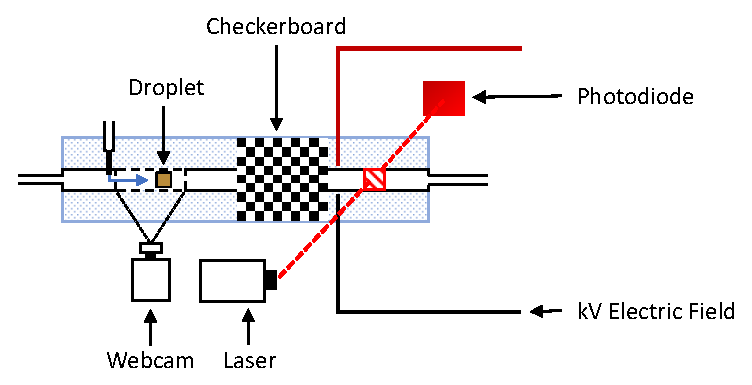
\includegraphics[scale=0.9]{Figures/Control.eps}
                    \caption{Figure to demonstrate the sealed chamber used to investigate continuously moving droplets. Into a slide consisting of PDMS, a cylindrical tunnel was created. Droplets were injected through the top port and flowed from left to right. After photographing a calibration checkerboard with a webcam, a small slice of this tunnel was selected and continuously monitored, and the size of passing droplets determined. The droplet was then oscillated with a variety of methods (in this case a small obstruction). Oscillations caused a laser beam directed at the tunnel to disperse, which was then detected with a photodiode.} 
                \label{fig:slide}
            \end{figure} 
    
        To move droplets through the slide, the 2 mm diameter capillary tubes were then connected to a fluid loop consisting of 3 mm diameter tubes, this is shown in Figure \ref{fig:basic}. To transport the spherical droplets, mineral oil of a lower viscosity was used as a carrier medium. A microfluidics motor was used to transport the oil from a central reservoir and around the loop. To reduce stress on the capillary tubes of the slide, the motor was attached on the "in" side, so oil was not being pulled against the external tubes, potentially breaking the connections. A t-junction was also placed at the return side of the loop to allow for simple bleeding of air. Droplets were then injected into this oil via the 1 mm port with a motorised syringe. After being interrogated in the slide, droplets were transported to the reservoir. Here, as the droplets were of different density to the mineral oil they would either sink or float and so they could be easily removed at a later point by hand. To prevent these droplets from returning into the flow system while still in the reservoir, the return and collection tubes were placed at different heights on opposite sides of the reservoir. This setup is demonstrated in Figure \ref{fig:basic}.
        
            \begin{figure}[H]
                \centering
                    \hspace*{2.0cm}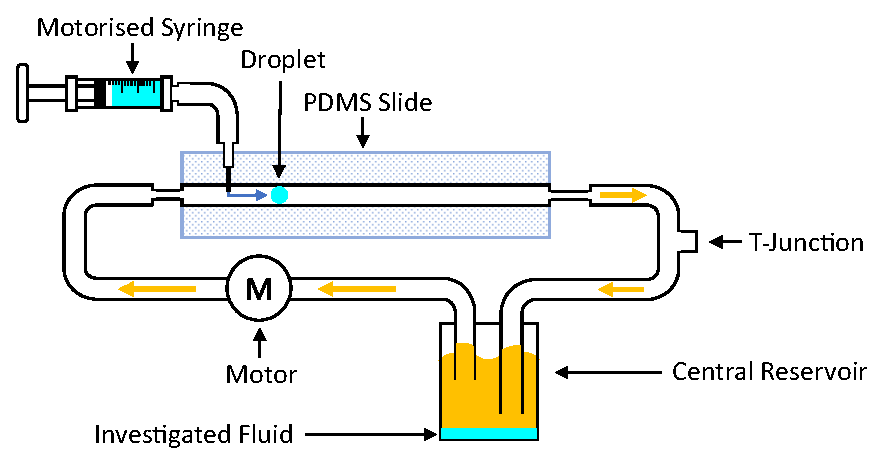
\includegraphics[scale=0.8]{Figures/Fluid.eps}
                    \caption{Figure to demonstrate the flow circuit used to investigate the rheological properties of droplets. Using a motor, a suspension fluid of mineral oil was transported from a central reservoir to a PDMS testing environment and back. A t-junction was placed in the back half of the loop to bleed air out of the system. A motorised syringe was used to suspend droplets of interest in the mineral oil, and subsequently investigated inside the PDMS slide. Droplets were then transported back to the reservoir, where they could be retrieved.} 	
                \label{fig:basic}
            \end{figure} 

    \subsection{Motor \& Syringe Pump\label{sect:method:motor}}

        To allow the speed of the fluid to programmatically controlled as part of the computer vision system discussed below, the motor had to be driven by a DAQ card. However, the DAQ card used lacked the circuitry to output sufficient current to drive the motor. Furthermore, the card had poor output resolution, making very fine control of fluid speed impossible. A current boosting circuit was therefore produced, and is shown in Figure \ref{fig:MotorCircuit}.  
        
            \begin{figure}[H]
                \centering
                \hspace*{-1.8cm}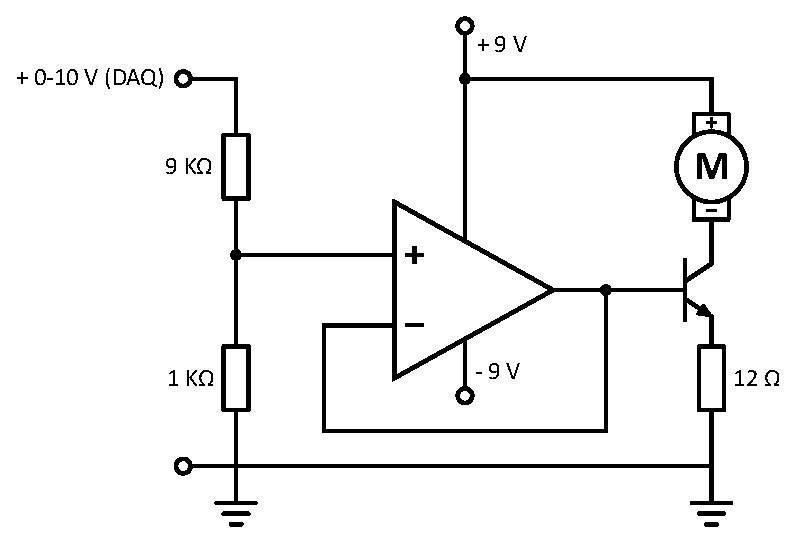
\includegraphics[scale=0.8]{Figures/MotorCircuit.eps}
                \caption{Circuit schematic of a circuit used to programmatically control the voltage applied to a motor. Depending on a 0-10 V signal from a DAQ card, between 0-4 V at 0-400 mA could be applied to the motor. This was required as the DAQ card alone was unable to produce sufficient current to drive the motor.}
                \label{fig:MotorCircuit}
            \end{figure}
        
        Besides using an external power supply to increase output current to suitable levels, it mapped the 0-4 V input rating of the motor to the full 0-10 V output of the DAQ, effectively increasing its sensitivity. This also allowed the very precise alteration of the voltage that the motor was running at. The resistances of the resistors were chosen both to provide the required output and provide good heat dissipation. Heat dissipation was further improved by attaching a heatsink to the transistor. The 12 $\Omega$ resistor was also replaced with 3 x 36 $\Omega$ resistors to reduce component stress. The motor was given protection by powering the circuit with a current limited power supply set at the maximum current rating of the motor. 
        
        To allow droplets of a consistent size of be created, a motorised syringe pump was set up, and code created to automatically interface over a COM port. To decrease the size of droplets being produced, the speed of the motor could be increased. However, droplets needed to be moved as slowly as possible to increase the time of data collection. Droplet size could therefore be made larger by increasing the speed at which the syringe pump was turned by writing code to interface with the pump through a serial port.
        
        
    \subsection{Determining Density\label{sect:method:density}}
    
        In previous experiments density, $\rho$, was typically calculated by using the radius, $R$, of each spherical droplet to determine its volume, $V$. The mass of the droplet, $m$, was then measured by absorbing a droplet onto a paper towel and comparing to the mass without the droplet\cite{hill}. This method is both destructive and erroneous by up to 10\%\cite{harrold2} due to mass loss during the experiment. It is also not viable for this project, as the droplets used in this project were suspended in fluid. Instead of measuring density per droplet, the density for the fluid in general was found. By holding the fluid of interest in a syringe, the mass of an empty and filled syringe could easily be compared to determine the mass of the fluid. The volume was then easily determined by reading from the scale of the syringe.
    
        This method had multiple advantages over other methods of determining the density. Firstly, it is non-destructive, making it more practical for many biological investigations such as protein crystallisation studies\textsuperscript{\cite{zhu}}, cell culture bio reactors\textsuperscript{\cite{konry}}, or any time where an expensive or rare liquid needs to be recovered\cite{Backholm2017}. Secondly, as the system was self contained and has all measurements taken within seconds there was no mass loss due to evaporation during the calculation of the density. Lastly, averaging down from larger volumes results in a lower percentage error per droplet which improved the accuracy of the measurement of the density.
        
    \subsection{Camera\label{sect:method:vision}}
        
        As the droplets in this project were not static, it was important that the programs written were efficient enough to analyse droplets before they exited the field of view of the camera. Furthermore, as MATLAB is an interpreted language and lacked hardware acceleration, webcam acquisition operatd at very low framerates. This made tracking moving droplets in real time difficult. This was overcome by using a package called Hebicam\cite{HebiCam}, which was originally created for streaming CCTV footage, and is a MATLAB wrapper for the more efficient openCV. After adapting it for use with USB webcams, 1080p video could be acquired at 30 FPS with spare processor overhead to perform calculations, as opposed to 6 FPS with none. To further improve the speed of calculations, images were not acquired in colour, but instead in greyscale. This also reduced the size of stored data. A Logitech C920 webcam was chosen as it had high image quality, high resolution, and a wide field of view with which to view droplets. 
            
        One of the major difficulties encountered during previous studies involved quickly computing the radius of droplets. Typically, previous authors first light the entire area around the droplet. They then count the width of the droplet in pixels, and convert this to the real world distance $R$ using simple trigonometry and the cameras focal length. This is as using computer vision with transparent droplets is extremely difficult, despite the common requirement of major industries such as oil separation to identify droplets during manufacturing\cite{bubblegeneral}. For one, without perfect, even lighting surrounding the droplet, droplets do not have bright regions of contrast fully around their boundary. Because the droplets are transparent, their centre looks identical to its surroundings, confusing simple algorithms\cite{bubblegeneral}. Droplets can also have bright reflections in their middle, adding even extra complexity. This is before considering the inevitable presence of noise in images. As such, more complex algorithms can take nearly a minute to run, yet still only achieve accuracies of approximately 80\%\cite{bubble2} when detecting droplets. We overcame these issues through use of background data to provide context.

        \subsubsection{Calibration\label{sect:method:vision:calib}}

            One of the major issues with only using the focal length of the camera to calculate $R$ is that this relies on the mistaken assumption that images are perfectly planar. Instead, non-linearities are introduced into images by distortions such as fish-eye in the camera. To ensure that droplet size was calculated accurately, checkerboard calibration was therefore applied. This first involves taking multiple photographs of a square checkerboard of known checker size at multiple positions in the field of view of the camera. It is then possible to algorithmically determine various extrinsic properties of the camera, such as its optical centre, distortions, and skew\cite{CameraCalibration}. As demonstrated in Figure \ref{fig:calibsetup}, knowledge of these extrinsic properties allowed for distortions in the lens to be accounted for. 
            
                \begin{figure}[H]
                    \centering
                    \begin{subfigure}[b]{0.48\textwidth}
                        \includegraphics[width=\textwidth]{Figures/Distorted.eps}
                        \caption{Before Calibration}
                        \label{fig:calibsetup:distorted}
                    \end{subfigure}
                    \begin{subfigure}[b]{0.48\textwidth}
                        \includegraphics[scale=1.27]{Figures/Undistorted.eps}
                        \caption{After Calibration}
                        \label{fig:calibsetup:undistorted}
                    \end{subfigure}
                    \caption{Figure }\label{fig:calibsetup}
                \end{figure}
            
            From here, $R$ could be calculated by taking an image of a droplet and a checkerboard, provided the droplet was in plane with the checkerboard. This is shown in Figure \ref{fig:slide}. The additional checkerboard was needed and had to be in plane with the droplet as the camera had no depth perception. Also, because the checkerboard did not move during experimentation, the checkerboard only had to be imaged once during each run of the experiment, provided that the setup did not move. This negated the need to calculate extrinsics after every droplet was observed, greatly improving efficiency. 
            
            There was an added complication to this process in that the PDMS used to create the experiment area was not perfectly flat. Because the algorithms worked on the assumptions that checkerboard was flat and the droplet was in plane with the checkerboard, significant errors would have been introduced if the checkerboard was glued to this uneven surface. The pattern was therefore instead printed on a long piece of paper, carefully folded and tensioned to the back of the slide. However, this resulted in a small 1mm disparity in depth between the droplet and the checkerboard, resulting in a small error. Using simple trigonometry to measure the distance to objects, this error was estimated to result in a 0.05 mm underestimation of all values of $R$, and as such was added to all calculated values of $R$. 
            
            Further, a limitation was placed on the maximum size of the checkerboard because the slide was of a finite size. Larger checkers had a lower percentage error from imperfect focusing, but smaller checkers could be placed in greater numbers. To determine the optimum checkerboard size for this project, the camera was calibrated with checkers between 1.50 and 5.00 mm in size and attempted to determine the size of circles of radius 0.10 to 1.00 mm, and accounted for the 0.05 mm offset. Ultimately, it was found most optimal to use checkers of size 0.20 x 0.20 mm in a 10 x 11 grid. 20 calibration images were then taken at different positions in similar positions to those used during this experiment. The positions of the checkerboard in the calibration screenshots as determined by the algorithm are shown in Figure \ref{fig:calib}. 
            
                \begin{figure}[H]
                    \centering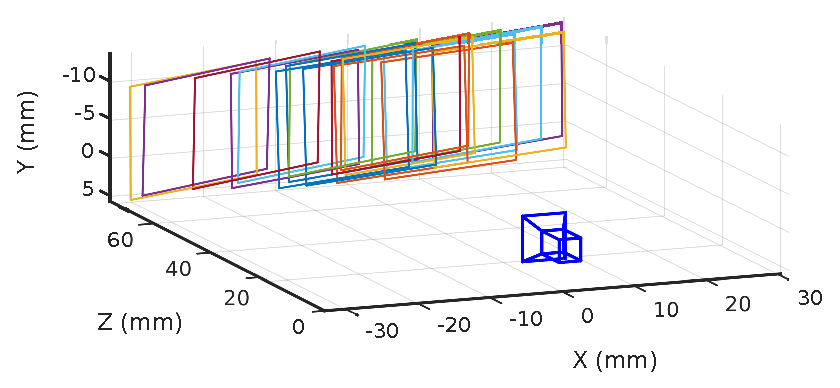
\includegraphics[scale=0.86]{Figures/CameraExtrinsics.eps}
                    \caption{Figure to demonstrate the multiple positions a checkerboard was placed in to calibrate a webcam. By taking multiple pictures of the checkerboard in multiple positions and knowing the size of the square checkers, the camera was be algorithmically calibrated to reliably determine object size. Because the positions of the checkerboard calculated by the algorithm agreed with the real-world placements, the camera was known to be accurately calibrated.}\label{fig:calib}
                \end{figure}
            
        \subsubsection{Determining Droplet Size\label{sect:method:vision:size}}
                
                After calibrating the camera, $R$ could then be determined by taking a photograph of the droplet. However, this was not possible while the droplets were moving. This was as photos would suffer from motion blur, and the droplets were slightly stretched while in motion. As such, the motor had to be stopped before taking a photo. This was done by continuously checking for the presence of a droplet in the slide. As the droplets were confined to a small area at any one time, only a small 3 mm long window of the slide was ever observed at one time to improve performance. The motor could therefore be stopped when a droplet was present within this small window. 
                
                To determine if a droplet was present, a background photo of the window was first taken with oil flowing but no droplet present as the syringe pump was not engaged. Every time a frame of video was captured, the window was subtracted from the corresponding background. Non-black pixels therefore corresponded to differences between the two photos. To increase the contrast of these difference in a non-linear manner, the contrast was multiplied by the arbitrarily selected log(6). When a droplet was present in the window, fully bright regions could be easily seen in the area where the droplet was. Once an arbitrary threshold of bright pixels was reached, the droplet was confirmed as being in the window, and the motor stopped. These steps are demonstrated in Figure \ref{fig:detector}.
            
                    \begin{figure}[H]
                        \centering
                        \begin{subfigure}[b]{0.3\textwidth}
                            
\includegraphics[width=\textwidth]{Figures/DropFinder/DropFinder1.eps}
                            \caption{Background}
                            \label{fig:detector:back}
                        \end{subfigure}
                        ~ 
                        \begin{subfigure}[b]{0.3\textwidth}
                            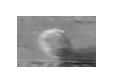
\includegraphics[width=\textwidth]{Figures/DropFinder/DropFinder2.eps}
                            \caption{Foreground}
                            \label{fig:detector:fore}
                        \end{subfigure}
                        ~ 
                        \begin{subfigure}[b]{0.3\textwidth}
                            
\includegraphics[width=\textwidth]{Figures/DropFinder/DropFinder3.eps}
                            \caption{Difference}
                            \label{fig:detector:diff}
                        \end{subfigure}
                        \caption{Figure to demonstrate how droplets were detected after being created by a mechanical pump. A region of the webcam was defined, and a background image taken (a). The region was then continuously monitored. If a droplet was present in the region (b), it could be detected by calculating the difference between (b) and (a) and multiplying by log(6). If enough bright pixels were observed (c), a droplet was known to be present in the system.}\label{fig:detector}
                    \end{figure}
            
            To reduce motion blur further, the system was thoroughly bled of air at all times. This is because air was the least dense medium present, and as it moved to the highest point in the system it pushed the oil and therefore the droplet. 
            
            Although this logical test to detect a droplet was sensitive to noise, it was chosen over a more accurate object finder as calculations had to be performed in under 1/30 of a second. Otherwise, the droplet could pass the window and fail to be detected, causing the entire system to fail. This noise meant that the carrier fluid had to be single coloured and free of impurities. 
            
            After stopping the motor and waiting for it to spin down, $R$ could then be calculated. A new photo was first taken of the droplet, which was now guaranteed to be in the pre-defined window, and its outline calculated. This was achieved with a 5-stage algorithm. First, the image was subtracted from the background as before to remove background detail. To bring out fine dark detail and reduce bright noise, a top-hat filter was then used to set all pixels with brightnesses below 10 to 0 (i.e. black), and all pixels with brightnesses above 20 to 255 (i.e. white). Of the remaining data, an automatic binarising algorithm was then applied to further bring out fine detail, and make a solid white horseshoe. This horseshoe was then turned into a convex hull and filled in. This shape could then be assumed to be a circle, and detected with a Circular Hough Transform based algorithm\cite{imfindcircles}. Each stage of this algorithm is shown in Figure \ref{fig:size}.
            
                \begin{figure}[H]
                    \centering
                    \begin{subfigure}[b]{0.3\textwidth}
                        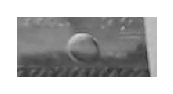
\includegraphics[width=\textwidth]{Figures/SizeFinder/SizeFinder1.eps}
                        \caption{Raw Image}
                        \label{fig:size:1}
                    \end{subfigure}
                    ~ 
                    \begin{subfigure}[b]{0.3\textwidth}
                        
\includegraphics[width=\textwidth]{Figures/SizeFinder/SizeFinder2.eps}
                        \caption{Background Subtraction}
                        \label{fig:size:2}
                    \end{subfigure}
                    ~ 
                    \begin{subfigure}[b]{0.3\textwidth}
                        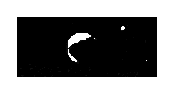
\includegraphics[width=\textwidth]{Figures/SizeFinder/SizeFinder3.eps}
                        \caption{Top Hat}
                        \label{fig:size:3}
                    \end{subfigure}
                
                    \begin{subfigure}[b]{0.3\textwidth}
                        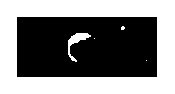
\includegraphics[width=\textwidth]{Figures/SizeFinder/SizeFinder4.eps}
                        \caption{Binarise}
                        \label{fig:size:4}
                    \end{subfigure}
                    ~ 
                    \begin{subfigure}[b]{0.3\textwidth}
                        
\includegraphics[width=\textwidth]{Figures/SizeFinder/SizeFinder5.eps}
                        \caption{Convex Hull}
                        \label{fig:size:5}
                    \end{subfigure}
                    ~  
                    \begin{subfigure}[b]{0.3\textwidth}
                        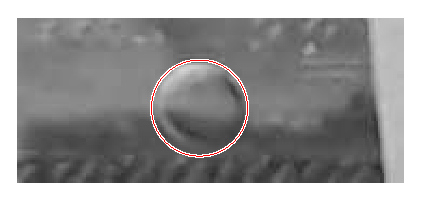
\includegraphics[width=\textwidth]{Figures/SizeFinder/SizeFinder6.eps}
                        \caption{Detected Circle}
                        \label{fig:size:6}
                    \end{subfigure}
                    \caption{Figure to demonstrate the method in which a bounding box could be drawn around a droplet to determine its size. After photographing the droplet (a), the photo could be subtracted from an image taken just before the droplet was present (b). A top hat filter was then applied to this droplet to remove noise (c), before thresholding to extract fine detail (d). The largest remaining horseshoe-shape could then be turned into a solid shape (e). As the droplet was assumed to be spherical, the bounding box of the droplet could then be found with a simple circular Hough transform (f) }\label{fig:size}
                \end{figure}
            
            After correcting this bounding box for fish-eye in the lens, the height and width. With knowledge of the perimeter of the droplet, a bounding box could be placed around each droplet, pixels converted to mm, and Equation \ref{eq:radii} used to determine the droplet radius. Once the size of the droplet was determined, the motor could be re-engaged to transport the droplet to the laser so that it can be analysed using the photodiode.
    
    \subsection{Oscillating Droplets\label{sect:method:oscillating}}
        
        After determining the size of the droplets, their vibrational spectra had to be determined. It was not possible to follow previous authors and induce vibrations with compressed air as the droplets were contained in a closed system. Magnetic coils were also considered, however this would have limited the approach to magnetic materials. Although the 30 Hz camera recording would not give enough data points to calculate the spectra, it was sufficient to observe oscillations. Vibrations were therefore confirmed to present if they they could be observed by eye with the camera. These were later confirmed with a 360 FPS phone camera.
        
        To induce oscillations, multiple methods were attempted. The first of these methods included the use of piezoelectric actuators and asymmetrically weighted vibration motors to vibrate the droplet. Secondly, the speed of the motor was changed to pulse rapidly to perturb the droplet using the control circuitry shown in Figure \ref{fig:MotorCircuit}. 
        
        A high voltage DC electric field was also considered. For reasons not thoroughly understood, it has been shown that a short, high voltage DC pulse passed across an unpolarised droplet can cause it to oscillate. As such, two exposed wires were dug into the PDMS on either side of the fluid channel, and each wire connected to either side of a 6 kV power supply to set up a simple circuit. Because of the high breakdown voltage of PDMS\cite{PDMSBreakdown} of 6 kV mm$^{-1}$, the electric field would be highly localised and directly through the channel. To maximise the strength of the electric field, the wires were dug into the PDMS as close to the fluid channel as possible. As the droplets moved through the channel and therefore through the field, they would therefore be subjected to a DC impulse. This allowed the power supply to be left on at all times, which was necessary as no equipment was available to switch the supply in the oscillation timescales required. 
        
        The final method in which oscillations were induced was to place a copper wire slightly inside the channel. This method relied on water having a high surface tension of around 70 mNm$^{-1}$, which is much higher than mineral oil at 30 mNm$^{-1}$. Water based droplets, amongst others, would therefore be inclined to cling to a new surface when brought nearby. The mineral oil with a much lower surface tension would not. This clinging is demonstrated in Figure X. However, as the droplet moved further away from the obstruction, its equilibrium would once again change to being spherical, and upon "pinging" back to this shape, would begin to oscillate. This made the droplet deform as it clung to the wire causing it to oscillate when freed. It was found that for numerous reasons stated in the discussion that for this project the obstruction in the channel was the best method to obtain results.
        
    \subsection{Laser \& Photodiode\label{sect:method:laser}}
    
        As the oscillations of the droplet were expected to occur at frequencies higher than the 30 FPS that the webcam could capture at, a photodiode was used to capture the intensity of a laser as it was refracted through the droplet. This set up is shown in Figure \ref{fig:slide}, with the laser on one side of the slide and the photodiode on the other. As the droplets in this project could be assumed to have a different refractive index to that of the carrier oil\cite{viscosity1,viscosity2}, it followed that the presence of a droplet would cause laser light to be scattered differently. Furthermore, as the shape of droplets varied as they oscillated, they caused light to scatter in proportion to their degree of oscillation. To prevent 50 Hz noise from an AC-DC power supply, the laser was driven by batteries.
        
        As droplets would be moving as they oscillated, the laser was broadly focused on a wide area of the slide. However, the laser was brightest about its centre and so the system would be more sensitive around this region than others. To improve the region of sensitivity, the solid angle of this bright region was increased by setting the laser up at a glancing angle of over 45$^{\circ}$ to the slide, instead of being face on. To further improve this situation, the laser was later replaced with a wider, more powerful He-Ne laser.
        
        To amplify the output of the photodiode to readable values, a simple circuit was set up\cite{artofelectronics}. A schematic of this circuit is shown in Figure \ref{fig:PDCircuit}. A variable resistor was used to act as a gain controller, allowing the output voltage to be made as high as possible within the 0-10 V recording range of the DAQ card. The 220 pF capacitor shown was not originally included, but was later added to reduce noise. A larger capacitor was considered as it would reduce more noise, however, it made the circuit less sensitive to small changes (i.e. oscillations).
    
        \begin{figure}[H]
            \centering
            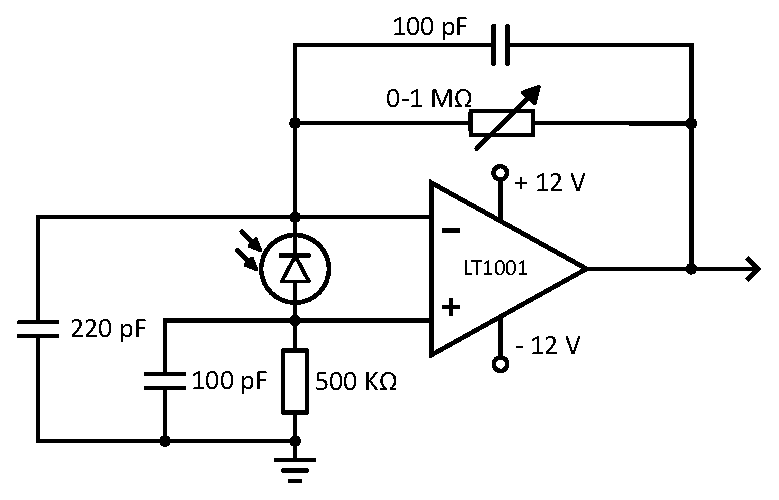
\includegraphics[scale=0.8]{Figures/PDCircuit.eps}
            \caption{Circuit schematic of a circuit used to amplify the reading of a photodiode used in the experiment. Extra smoothing is applied in the form of a 220 pF capacitor, and amplification gain is set by the resistance of a 1 M$\Omega$ variable resistor.}
            \label{fig:PDCircuit}
        \end{figure}
    

    \subsection{Running Experiments\label{sect:method:exp}}
        
        Through the running of a user-friendly toolbox, which required minimum setup, droplets were rapidly interrogated. To set up the code and equipment, files and folders were first automatically created to store raw data. At this point, a previous camera calibration could be selected, or if so desired a new one created with a chooseable number of images. After approving this calibration, operating parameters such as motor voltage and photodiode recording time were then defined. The DAQ card, pump and webcam were then interfaced with so they could be controlled. At this point, the camera was imaged, the checkerboard found, and camera extrinsics calculated. The window of the webcam image in which the droplet was to be imaged was then selected. These setup steps are shown in Figure \ref{fig:setup:flow}.
        
        \newpage
        \begin{figure}[H]
            \centering
            \hspace*{-5.4cm}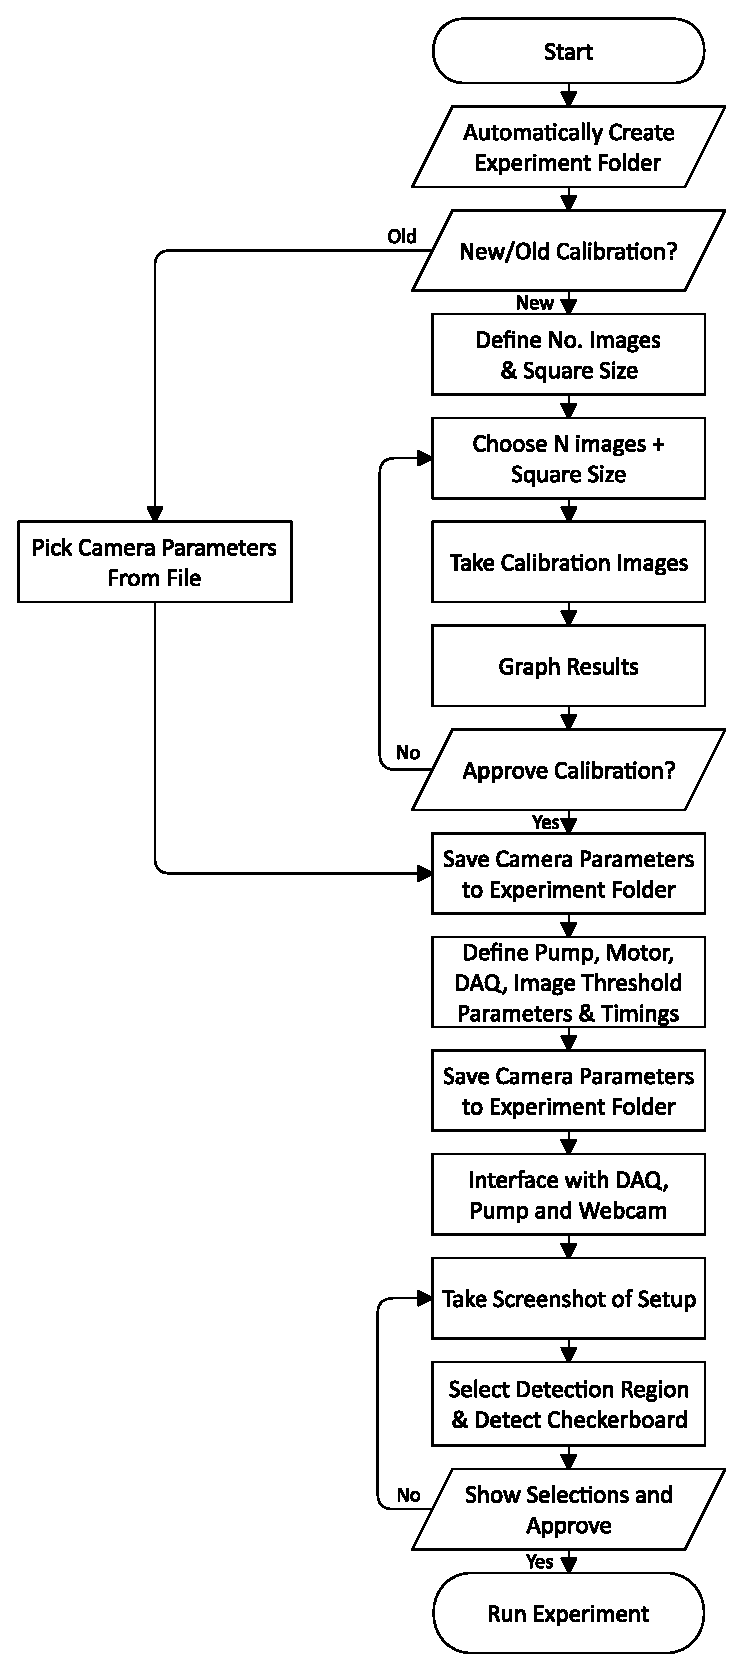
\includegraphics[scale=0.8]{Figures/FlowSetup.eps}
            \caption{Flow chart to demonstrate the process by which the system could be set up to allow for the automated measuring of rheological properties of droplets.}
            \label{fig:setup:flow}
        \end{figure}
        
        From here, no further user input was required, and experiments were automatically run. As shown in Figure \ref{fig:setup:logic}, this first began with turning on the motor and running it for a few seconds to clear out any stray material from the slide. The detection window defined earlier was then imaged, and the background image shown in Figure \ref{fig:detector:back} taken. The syringe pump was then turned on for just long enough to produce a single droplet of a consistent size. A video was then taken of the window in real time, and after every frame the foreground was subtracted from the background and compared. Once the threshold conditions described in Section \ref{sect:method:vision:size} were met, the motor was stopped, distortions accounted for, and the size of the droplet found. The motor was then re-engaged, and the photodiode spectrum recorded. After a pre-defined amount of time, oscillations were detected in this spectrum by looking for significant changes in the signal, and this area Fourier Transformed. The Fourier Transform could then be calculated, along with $f$ and $\Delta f$. This data was then saved to disk. Extra droplets could then be produced to produce further results.
    
        \begin{figure}[H]
            \centering
            \hspace*{-1cm}\includegraphics[scale=0.8]{Figures/FlowLogic.eps}
            \caption{Flow chart to demonstrate the control logic used by the system to automatically measure the rheological properties of droplets.}
            \label{fig:setup:logic}
        \end{figure}

\section{Error Analysis} 
    
    There were several major sources of error in the project. When calculating the mass of the liquid, an error was produced when comparing the difference in mass between a filled and empty syringe. As such, the precision of the measuring scale, 0.001 g, was added in quadrature with itself. There was also an error on the volume of the syringe, which was defined as the precision of the scale, 0.2 mL. These two errors were propagated together to determine the error on the density of the droplet.
    
    Furthermore, there were several sources of error involved when calculating $R$. Firstly, there was the mean error of 0.41 $\pm$ 0.02 pixels across the 20 calibration images when calibrating the camera, which would turn into an error when converting between pixel space and real space. However, as the bounding box finding algorithm only operated to a per-pixel accuracy, this sub-pixel error was negligible. This was seen when calculating the size of known objects, which was found to have an average standard deviation of 0.03 mm away from the expected size. This is shown in Figure \ref{fig:calib:error}. 
        
            \begin{figure}[H]
                \centering
                \hspace*{-1cm}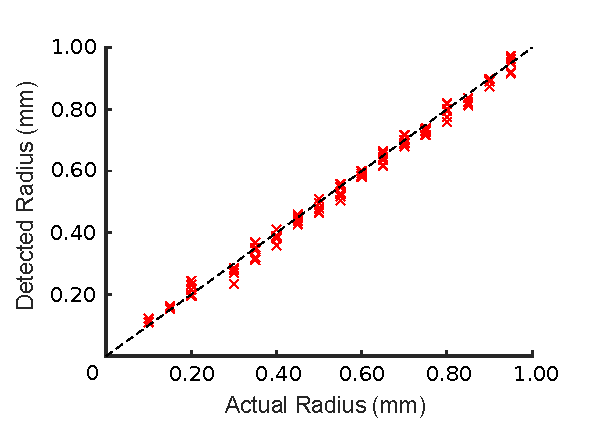
\includegraphics{Figures/CameraCalib.eps}
                \caption{Figure to demonstrate the accuracy by which a calibrated webcam could calculate the radius of multiple bright circles of known size. Given the small standard deviation of 0.03 mm from expected values and strong linear agreement across multiple radii, it can be seen that the calibration and size calculation algorithms used in the experiment worked as intended.}
                \label{fig:calib:error}
            \end{figure}
    
    Additionally, there was also an error due to the imperfect finding of the bounding boxes around the droplet. By comparing the bounding boxes of 20 droplets drawn by hand and by algorithm, 100\% of the droplets were detected by the algorithm to within $\pm$2 pixels in radius. As the droplets had diameters of around 80 pixels, it was estimated that the boundary of a droplet could be calculated to within a 5\% error. 5\% of $R$ was therefore added in quadrature with the 0.03 mm discussed above to calculate the final error on $R$. 
    
    The errors on $f$ and $\Delta f$ were also considered. The error on $f$ was defined as the resolution of the frequency axis of the Fourier Transformed signal. The error on $\Delta f$ was similarly defined as the error on $f$ added in quadrature with itself. Ultimately, the errors on $\rho$, $R$, $f$ and $\Delta f$ were propagated through Equations \ref{eq:SurfaceTension} and \ref{eq:Viscosity} to calculate final errors.
    
    Ultimately, the largest source of error in Equations \ref{eq:SurfaceTension} and \ref{eq:Viscosity} was considered to be the small amount of time that oscillations could be recorded for. This was because frequency resolution was a function of both sampling rate and sample time, but sampling rate could not be reliably increased past 3000 Hz without causing equipment errors. As such, the lowest possible frequency resolution was set by the time that oscillations could be detected for. As discussed below, oscillations could often only be detected for 0.5 seconds. In these case, the frequency resolution would be as low as 2-3 Hz, or approximately 30\% of the observed value of $f$. Furthermore, as Equations \ref{eq:SurfaceTension} and \ref{eq:Viscosity} were both a second order of function of $f$ and $\Delta f$, substantial errors could be produced. 
    
\section{Results \& Discussion}

\subsection{Unsuspended Water}
 	
        To determine an idea of the frequency that was expected for water droplets used in this project an experiment was conducted with a sessile water droplet. The sessile water droplet was blown on to give it the impulse needed to start oscillating. It can be seen from Figure \ref{fig:Water} that blowing on the droplet produced clear oscillations for around 2.5 seconds. This indicated that oscillations should be visible for at least this length of time to produce results comparable with the original method. Once Fourier Transformed it was observed that the oscillations were at a frequency of approximately 10 Hz. From this it was known that a similar frequency for the water droplets suspended in mineral oil could be expected. This experiment also confirmed that the set up was working as expected as this gave very similar results to a paper by Temperton et al\cite{Temperton2012}. 
 
            \begin{figure}[H]
            \centering
                    \begin{subfigure}[b]{0.48\textwidth} \hspace*{0cm}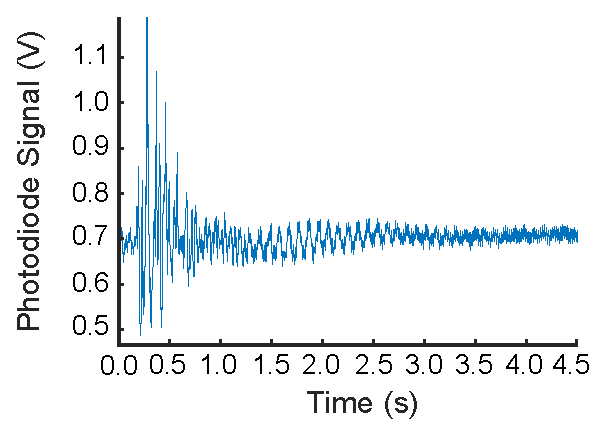
\includegraphics[width=\textwidth]{Figures/WaterSignal.eps}
                    \caption{Original Signal}
                    \label{fig:Water:Signal}
                \end{subfigure}\hspace{3pt}
                \begin{subfigure}[b]{0.48\textwidth}
                    \hspace*{0.1cm}\includegraphics[width=\textwidth]{Figures/WaterSignalPD.eps}
                    \caption{Fourier Transform}
                    \label{fig:Water:FT}
                \end{subfigure}
            \caption{Plot to demonstrate (a) the original signal, and (b) the resulting Fourier Transform of a standing droplet in air vibrated with a pulse of air.}\label{fig:Water}
            \end{figure} 

    \subsection{Control Equipment}
    
        Using the circuit shown in Figure \ref{fig:MotorCircuit}, we can easily change the voltage that the motor was ran at. As can be seen by Figure \ref{fig:MotorCalib}, the motor voltage increases linearly with the voltage outputted through the DAQ card. As we used a current limiting power supply it was seen that once the motor voltage increased above 4 V, increasing the DAQ voltage further did not increase the motor voltage above 6 V. Using this graph the current that used by the motor at each voltage can easily be calculated as the internal resistance of the motor was 10 $\Omega$.
        
        Oh yeh, what's the density of water?
        
        \begin{figure}[H]
            \centering
            \hspace*{-1cm}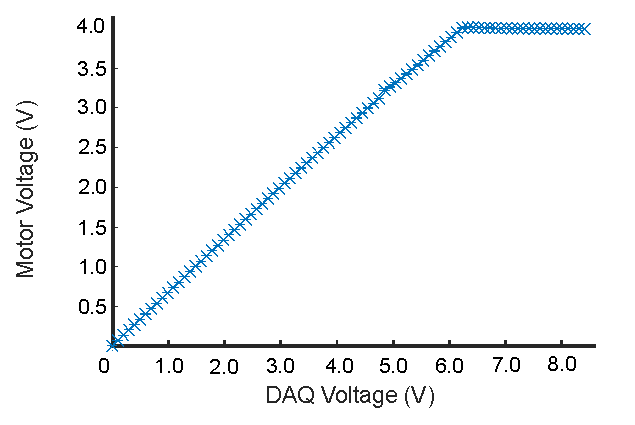
\includegraphics{Figures/MotorCalib.eps}
            \caption{Figure to demonstrate the output voltage provided to a motor by a current boosting circuit, depending on its input voltage. A current limiter was also attached to prevent overvolting the motor. This was created to allow a 2-4 V, 200-400 mA motor to be programmatically driven by a 0-10 V DAQ card without the capability to output current. As it outputs the correct voltages and currents until the clearly visible current limit, the circuit can be considered to be working correctly.}\label{fig:MotorCalib}
        \end{figure}
        
        As there was a strong agreement between expected and detected circle values, seen in Figure \ref{fig:calib:error}, it can be seen that the size finder algorithm worked as intended. However, the algorithm struggled to detect circles under a radius of 0.30 mm, and hence, there was a lower limit to the size of the droplet that could be analysed in this project.
        
        To observe oscillations for the longest period of time possible we ran the motor at 1.5 V. This was the lowest voltage that the motor ran at and hence, the slowest speed that the droplet could travel through the slide. By measuring the length of the slide and the time taken for a droplet to travel through the droplet we determined that the droplet travelled throughout the slide at 0.004 ms$^{-1}$.  
        
    \subsection{Oscillating Droplets}
      
        To try and oscillate the droplets four different methods were tried. It was found that using an obstruction in the channel to perturb the droplets was the best method, in this project, to obtain results. However, initially the use of piezoelectric actuators and asymmetrically weighted vibration motors was considered. However, these had to be attached externally to the slide and therefore made the slide as a whole vibrate (if at all) and not only the droplet within as desired. Hence, any oscillations of the droplets were not detectable over the noise coming from the entire slide also vibrating.
        
        Secondly, an attempt to induce oscillations by changing the speed of the motor using the control circuitry shown in Figure \ref{fig:MotorCircuit} was used. Although the motor could have been pulsed rapidly, this was akin to driving the droplets at a single frequency, rather than applying an impulse. This was confirmed by the presence of a single peak at the frequency that the motor was pulsed. Instead, oscillations were attempted to be induced by applying one sudden change in motor voltage, with the hope of having the sudden change in velocity cause the droplet to stretch horizontally and therefore induce oscillations. This was unsuccessful as the applied force by the change of velocity was too weak to induce any measurable oscillations.
        
        At this point, a DC electric field was used to oscillate the droplets. however, this was not viable. This noise is shown in Figure \ref{fig:control}. 
        
        \begin{figure}[H]
            \centering
            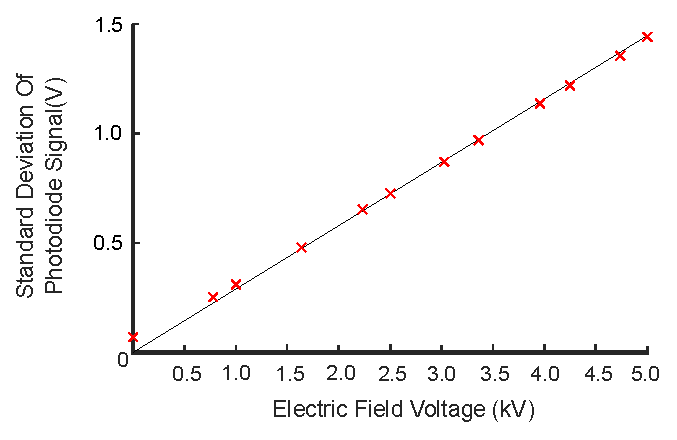
\includegraphics{Figures/ElecFieldNoise.eps}
            \caption{Figure to demonstrate the noise produced in a photodiode circuit produced by the presence of a high voltage power supply. As there is a linear relationship, the noise is clearly the fault of the supply/wires, and is the reason why the electric field could not be used to produce oscillations.} 	
            \label{fig:control}
        \end{figure} 
        
        It can be seen from this graph that the electric field voltage was directly proportional to the standard deviation of the photodiode signal. It could therefore be concluded that the source of the noise was the high voltage power supply. It is likely that this noise was due to stray magnetic fields being produced. To reduce the wires producing stray magnetic fields and causing interference in the photodiode circuit by Lenz Law, all wires were tightly twisted in pairs. The photodiode circuit was also recreated to fit the small size of a grounded metal box. Although this decreased noise significantly, the noise was still too large.        Because late timescale oscillations could be as low as 0.2 V, the noise from the power supply would swamp out the signal produced by oscillations. Use of a DC electric field was therefore not a viable option. This was compounded further by the fact that an electric field voltage of over 3.0 kV was needed to see any visible oscillations. 
        
        Finally, a wire obstruction was pushed into the slide. This is shown in Figure \ref{fig:slide}. Starting from a sharp "ping" when the droplet detached from the needle, oscillations could be clearly detected. This is shown in Figure \ref{fig:oscillation}. When qualitatively comparing this typical signal with the expected signal from Figure \ref{fig:temperton:signal}, both signals have similar shapes and timescales, giving further indication of success. Although an exponential decay should be present in an oscillatory signal, its absence is easily understood. As the laser was not uniform, the amplitude of the signal due to the oscillations of the droplet, was found to be dependant on the position of the droplet within the laser beam. 
        
         \begin{figure}[H]
            \centering   
            \begin{subfigure}[b]{0.48\textwidth}
                \hspace*{0cm}\includegraphics[width=\textwidth]{Figures/PingSignal.eps}
                \caption{Original Signal}
                \label{fig:oscillation:signal}
            \end{subfigure}\hspace{3pt}
            \begin{subfigure}[b]{0.48\textwidth}
                \hspace*{0.1cm}\includegraphics[width=\textwidth]{Figures/PingPD.eps} 
                \caption{Fourier Transform}
                \label{fig:oscillation:FT}
                \end{subfigure}
            \caption{Figure }\label{fig:oscillation}
        \end{figure} 
        
        After Fourier transforming this signal, a significant peak could be observed at approximately 10 Hz. Further, the peak was lorentzian in shape. This was in agreement with the expected value from Figure \ref{fig:Water:FT}, giving evidence that the signal acquired was indeed due to oscillations. It is therefore possible to oscillate moving droplets with an obstruction.
        
        It could also be seen in Figure \ref{fig:oscillation} that the algorithm for determining the section of the photodiode signal when oscillations were present was also clearly successful, as it determined a section of the signal where oscillations were present. This is shown in the figure as the blue section of the signal. It can therefore also be concluded that it is viable to automate the process of determining the rheological properties of droplets.
        
        However, when using the high speed camera it was observed that the oscillations were of lower magnitude and shorter timescale compared to using the DC electric field. To capture the signal graphed above, several changes had to be made. To increase the strength of the "ping" (and therefore of the oscillatory signal), the droplet had to be made to cling more strongly to the obstruction. The obstruction material was considered, and from a syringe needle, nickel plated wire and copper plated wire, more promising results were seen with the copper. The obstruction was also roughed up with sandpaper to increase its surface area. A polarising charge was then introduced to the obstruction by oxidising it. A Van-der-Graff generator was also considered to polarise the obstruction, increasing attraction strength further. However, applying a charge when the droplet was nearby caused the droplet to break apart. As the speed of droplets could never be known precisely, it was also not possible to use timing circuits for the dissipation of charge. We also considered the height of the obstruction with respect to the amplitude of oscillations. When the obstruction was deeper into the channel, droplets would be more likely to break up, whilst shallower obstructions would result in oscillations of lower magnitude. The obstruction was therefore placed two thirds of the way into the tunnel.
        
    \subsection{Calculating $\eta$ and $\gamma$}
    
        \begin{figure}[H]
            \centering   
            \begin{subfigure}[b]{0.48\textwidth}
                \hspace*{0cm}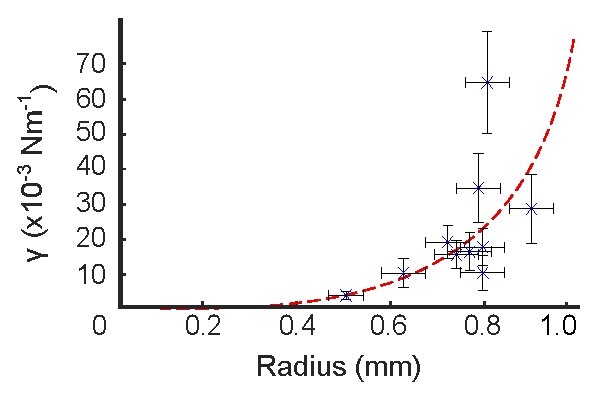
\includegraphics[width=\textwidth]{Figures/r_vs_gamma.eps}
                \caption{Original Signal}
                \label{fig:vsgamma:r}
            \end{subfigure}\hspace{3pt}
            \begin{subfigure}[b]{0.48\textwidth}
                \hspace*{0.1cm}\includegraphics[width=\textwidth]{Figures/f_vs_gamma.eps} 
                \caption{Fourier Transform}
                \label{fig:vsgamma:f}
                \end{subfigure}
            \caption{Figure }\label{fig:vsgamma}
        \end{figure} 
     
        \begin{figure}[H]
            \centering   
            \begin{subfigure}[b]{0.48\textwidth}
                \hspace*{0cm}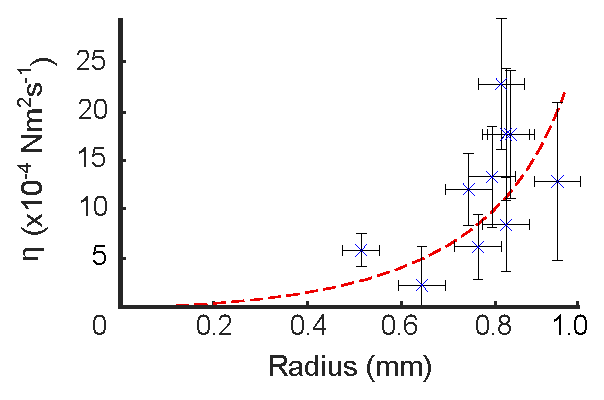
\includegraphics[width=\textwidth]{Figures/r_vs_eta.eps}
                \caption{Original Signal}
                \label{fig:vseta:r}
            \end{subfigure}\hspace{3pt}
            \begin{subfigure}[b]{0.48\textwidth}
                \hspace*{0.1cm}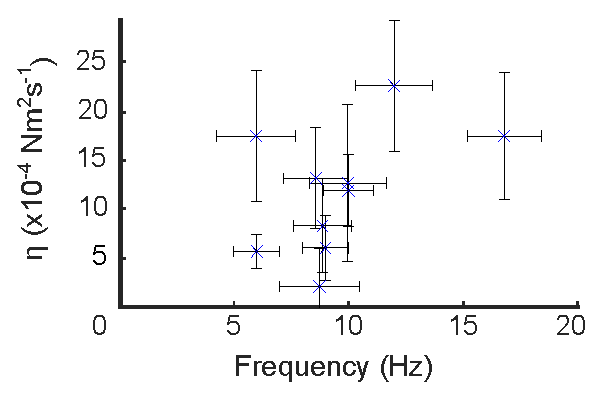
\includegraphics[width=\textwidth]{Figures/f_vs_eta.eps} 
                \caption{Fourier Transform}
                \label{fig:vseta:f}
                \end{subfigure}
            \caption{Figure }\label{fig:vseta}
        \end{figure} 
        
        \begin{figure}[H]
            \centering
            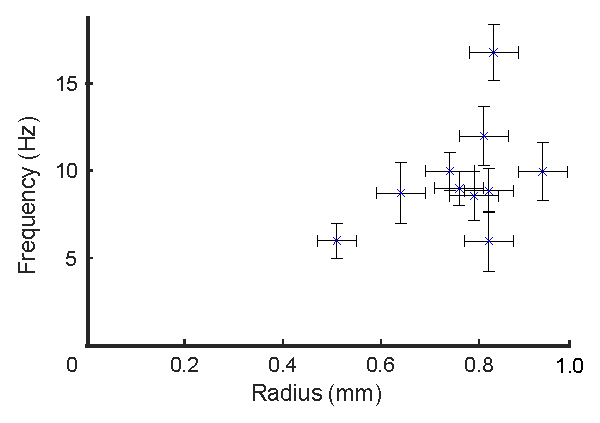
\includegraphics{Figures/r_vs_f.eps}
            \caption{Figure .} 	
            \label{fig:rvsf}
        \end{figure} 
        
        
\section{Limitations \& Future Improvements}
    
    Some limitation of this project included that the Matlab code was written to automatically interface with the pump over a COM port. This has a significant delay, reducing the throughput of droplets in the fluidic system.
    
    There were a few drawbacks to this algorithm. For one, it was highly sensitive to noise, meaning that if the oil is cloudy then it will fail. The top-hat filter was also semi-manual, and must be tweaked for different droplet colours/transparencies. It also struggles with droplets with a radius below 0.3 mm. Finally, it also relies on the assumption that the droplets are perfectly spherical, which is not completely true.
    
    The camera itself also had several drawbacks. When measuring $R$, errors were largely due to the pixel-level precision and small number of pixels taken up by the droplet. As the droplets produced for the experiment were typically around 25 pixels in radius, they only took up 2000 of the 2073600 pixels in a 1920 x 1080 image, only around 0.1\% of the pixels of the image. If the camera had a lower focal length, it could be positioned far closer to the droplet, allowing droplets to take up a higher percentage of the pixels in the image allowing for much better image detection. This would result in a significantly smaller error in the droplet size calculator. Another method to decrease this error would be to use a higher resolution camera as it would also increase the accuracy of boundary detection due to the larger number of pixels detected in the droplet. However, this would decrease the efficiency of the program, potentially causing it to lose frames. As such, the need to track droplets in real time with a camera could be completely negated by using another laser and photodiode to act as a "trip" switch. When a droplet is present, there would be a rapid change in the photodiode signal. The motor could then be stopped, and the droplet imaged as before, with no performance penalty for increasing resolution.
    
    One of the largest limitations to investigating moving droplets was that of short signal times. Because oscillations could only be observed when the droplet was in the path of the laser beam, the effectiveness of the system was highly bound by the correct position of the laser relative to the obstruction. The effectiveness of the system was therefore incredibly sensitive to the position of the laser, with laser movements of 2 - 3 mm being sufficient to render the oscillation unrecordable. This sensitivity was the reason why optimising obstruction material, obstruction height, laser angle and laser positions could only be achieved in a qualitative fashion. 
    
    Further, the timescales that signals could be recorded appeared to decrease significantly during the experiment. Initially, oscillatory signals were typically visible for 1 - 1.5 seconds. However, for the results captured for Section X, despite the improved capture location, oscillations were only visible for less than 0.5 seconds, if at all. This may have been due to decreasing performance of the photodiode used. Although the noise did not change as it was due to the circuit, the photodiode may have become less sensitive, meaning that only the strongest oscillations were visible. This could not be observed with signal intensity, as this was dependant on the gain of the photodiode circuit and the position of the photodiode relative to the laser beam. Future experimentation should therefore be aware of it going to shit.  
    
    In this project it has been shown that droplets can be made to reliably oscillate using a high-throughput fluidic system and hence, future work should focus around refining methods to observe these oscillations. If high speed, high voltage switching equipment was available, the electric field could be turned off when recording from the photodiode, negating the issues related to stray magnetic fields. Further, a more powerful laser or laser with a much wider beam could be used. This would allow oscillations to be observed with a greater amplitude, in the case of a more powerful laser, or for a longer period of time, for a wider beam. 
    
    Another method that could be used to detect oscillations for longer periods of time is to use either a larger photodiode or a wide array of photodiodes and add up the signal from each one. MENTION THE GLASS ROD? An avalanche photodiode could also be used to be even more sensitive to the variations in the signal related to the oscillations. To do this however, the laser that is used must be incredibly stable or the noise detected would be far too large to detect any of the oscillations. A slower motor than the one available for this experiment could be used, or the computer vision code extended to fully stop a droplet once it began oscillating.
    
    Alternatively, make the detection of oscillations much simpler would to be to use an adjustable focus high speed camera rather than using a laser. This is because it would remove all of the concerns about the noise if a reliable shape and size finder algorithm could be developed. This would also remove all concerns about not being able to detect the oscillations for long enough as droplets would be able to be tracked over the entire length of the slide which would be easily long enough to determine the frequency of oscillation. 
    
    One of the reasons a high-throughput fluidic system was developed was so that droplets could be analysed using a non destructive technique. However, due to time constraints a system to reliably extract the droplets from the oil once they had gone round the system was not developed in this project. Hence, future studies could try to develop a system to extract the droplets so that they can be put through the system again and re-analysed.
    
    Errors could also be improved. To reduce the frequency step in a Fourier Transform and therefore decrease the errors, both the time of the signal and the sampling rate can be increased. A maximum bound was therefore set based on the maximum time that the droplets would oscillate. Although the DAQ card could theoretically sample at higher than the 2000 Hz experiments were sampled at, various errors occurred when attempting to do so.
    
    

\section{Conclusions}

% -----------
% REFERENCES
% -----------
\newpage
\bibliographystyle{unsrt}
\bibliography{references}

% -----------
% CODE
% -----------
\newpage
\appendix{}
\section{Code}
% -----------
% FIN
% -----------
\end{document}    